\documentclass[aspectratio=169]{beamer}
\usepackage{will_handley_beamer}
\usepackage{title_page}

% Commands
% --------
% - \arxiv{arxiv number}
% - \arxiv{<number>}            arxiv.org/abs/<number>
% - \oldarxiv{<arxiv number>}   arxiv.org/<number>
% - \doi{<doi>}                 doi.org/<doi>
% - \xkcd{<number>}             xkcd.com/<number>
% - \email{<email>}             <<email>>
% - \tthref{<website>}          <website>
% - \av[dist]{<quantity>}       <quantity>_{dist}
% - \student{<name>}{<detail>}{<photo>}

% Talk details
% ------------
\title{GPU-native nested sampling in BlackJAX}
\subtitle{Accelerating Bayesian inference to state-of-the-art levels}
\date{<+Date+>}

\begin{document}

\begin{frame}
    \titlepage
\end{frame}

\begin{frame}
    \frametitle{What is Nested Sampling?}
    \begin{itemize}
        \item Nested sampling is a radical, multi-purpose numerical tool.
        \item Given a (scalar) function $f$ with a vector of parameters $\theta$, it can be used for:
    \end{itemize}
    \vspace{-10pt}
    \begin{columns}[t]
        \column{0.3\textwidth}
        \begin{block}{Optimisation}
            \[\theta_\text{max} = \max_\theta{f(\theta)}\]
        \end{block}
        \column{0.3\textwidth}
        \begin{block}{Exploration}
            \vspace{-10pt}
            \[\text{draw/sample}\quad \theta\sim f\]
            \vspace{-15pt}
        \end{block}
        \column{0.3\textwidth}
        \begin{block}{Integration}
            \[\int f(\theta) dV \]
        \end{block}
    \end{columns}
    \begin{columns}[t]
        \column{0.33\textwidth}
        \centerline{\includegraphics[width=0.8\textwidth,page=13]{figures/himmelblau}}
        \column{0.33\textwidth}
        \centerline{\includegraphics[width=0.8\textwidth,page=15]{figures/himmelblau}}
        \column{0.33\textwidth}
        \centerline{\includegraphics[width=0.8\textwidth,page=14]{figures/himmelblau}}
    \end{columns}
\end{frame}

\begin{frame}
    \frametitle{Where is Nested Sampling?}
    \begin{columns}
        \column{0.5\textwidth}
        \begin{itemize}
            \item For many purposes, you should group Nested Sampling with (MCMC) techniques such as:
                \begin{itemize}
                    \item Metropolis-Hastings (PyMC, MontePython)
                    \item Hamiltonian Monte Carlo (Stan, \textbf{blackjax})
                    \item Ensemble sampling (emcee, zeus). 
                    \item Variational Inference (Pyro)
                    \item Sequential Monte Carlo 
                    \item Thermodynamic integration
                    \item Genetic algorithms
                \end{itemize}
            \item You may have heard of it in branded form:
                \begin{itemize}
                    \item MultiNest
                    \item PolyChord
                    \item dynesty
                    \item ultranest
                \end{itemize}
            \end{itemize}
        \column{0.5\textwidth}
        \begin{columns}
            \column{0.5\textwidth}
        \includegraphics[width=\textwidth]{figures/emcee}
        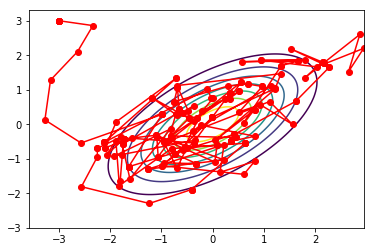
\includegraphics[width=\textwidth]{figures/metropolis-hastings}
            \column{0.5\textwidth}
        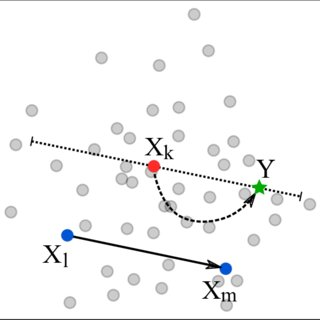
\includegraphics[width=\textwidth]{figures/zeus}
        \end{columns}
        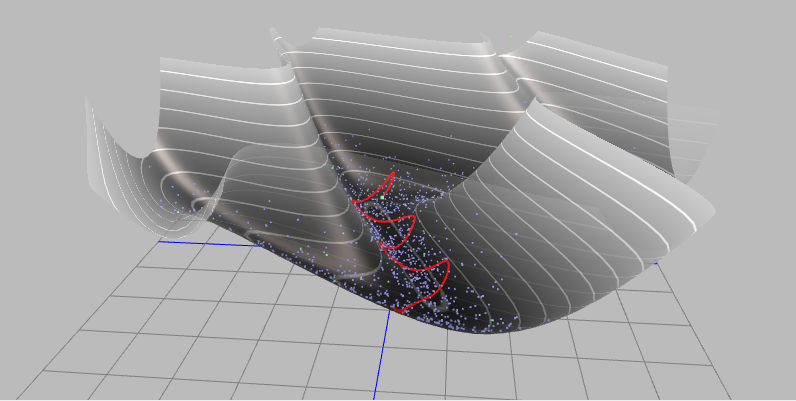
\includegraphics[width=\textwidth]{figures/hmc_explained}
    \end{columns}
\end{frame}

\begin{frame}
    \begin{columns}
        \column{0.48\textwidth}
        \begin{block}{\textbf{MCMC}}
            \only<16>{
                \begin{itemize}
                    \item Single ``walker''
                    \item Explores posterior
                    \item Fast, if proposal matrix is tuned
                    \item Parameter estimation, suspiciousness calculation
                    \item Channel capacity optimised for generating posterior samples
                \end{itemize}
            }
        \end{block}
            \includegraphics<1>[width=\textwidth,page=1]{figures/himmelblau_mcmc}%
            \includegraphics<2>[width=\textwidth,page=2]{figures/himmelblau_mcmc}%
            \includegraphics<3>[width=\textwidth,page=3]{figures/himmelblau_mcmc}%
            \includegraphics<4>[width=\textwidth,page=4]{figures/himmelblau_mcmc}%
            \includegraphics<5>[width=\textwidth,page=5]{figures/himmelblau_mcmc}%
            \includegraphics<6-15>[width=\textwidth,page=9]{figures/himmelblau_mcmc}%
        \centerline{\includegraphics<16>[width=0.5\textwidth,page=9]{figures/himmelblau_mcmc}}
        \column{0.48\textwidth}
        \begin{block}<7->{\textbf{Nested sampling}}
            \only<16>{
                \begin{itemize}
                    \item Ensemble of ``live points''
                    \item Scans from prior to peak of likelihood
                    \item Slower, no tuning required
                    \item Parameter estimation, model comparison, tension quantification
                    \item Channel capacity optimised for computing partition function
                \end{itemize}
            }
        \end{block}
            \includegraphics<7|handout:0>[width=\textwidth,page=1]{figures/himmelblau}%
            \includegraphics<8|handout:0>[width=\textwidth,page=2]{figures/himmelblau}%
            \includegraphics<9|handout:0>[width=\textwidth,page=3]{figures/himmelblau}%
            \includegraphics<10          >[width=\textwidth,page=4]{figures/himmelblau}%
            \includegraphics<11|handout:0>[width=\textwidth,page=5]{figures/himmelblau}%
            \includegraphics<12|handout:0>[width=\textwidth,page=6]{figures/himmelblau}%
            \includegraphics<13|handout:0>[width=\textwidth,page=7]{figures/himmelblau}%
            \includegraphics<14|handout:0>[width=\textwidth,page=8]{figures/himmelblau}%
            \includegraphics<15|handout:0>[width=\textwidth,page=15]{figures/himmelblau}%
        \centerline{\includegraphics<16>[width=0.5\textwidth,page=4]{figures/himmelblau}} 
    \end{columns}
\end{frame}

\begin{frame}
    \frametitle{The nested sampling meta-algorithm: live points}
    \begin{columns}
        \column{0.5\textwidth}
        \begin{itemize}
            \item Start with $n$ random samples over the space.
            \item Delete outermost sample, and replace with a new random one at higher integrand value.
            \item The ``live points'' steadily contract around the peak(s) of the function.
            \item We can use this evolution to estimate volume \emph{probabilistically}.
            \item At each iteration, the contours contract by $\sim\frac{1}{n}\only<5->{\pm \frac{1}{n}}$ of their volume.
            \item This is an exponential contraction, so
                \[  \int f(x) dV \approx \sum_i f(x_i) \Delta V_i, \quad V_i = V_0 e^{-\only<5->{(}i\only<5->{\pm\sqrt{i})}/n} \]
        \end{itemize}
        \column{0.5\textwidth}
        \includegraphics<1|handout:0>[width=\textwidth,page=1]{figures/himmelblau}%
        \includegraphics<2|handout:0>[width=\textwidth,page=2]{figures/himmelblau}%
        \includegraphics<3|handout:0>[width=\textwidth,page=3]{figures/himmelblau}%
        \includegraphics<4-         >[width=\textwidth,page=4]{figures/himmelblau}%
    \end{columns}
\end{frame}

\begin{frame}
    \frametitle{The nested sampling meta-algorithm: dead points}
    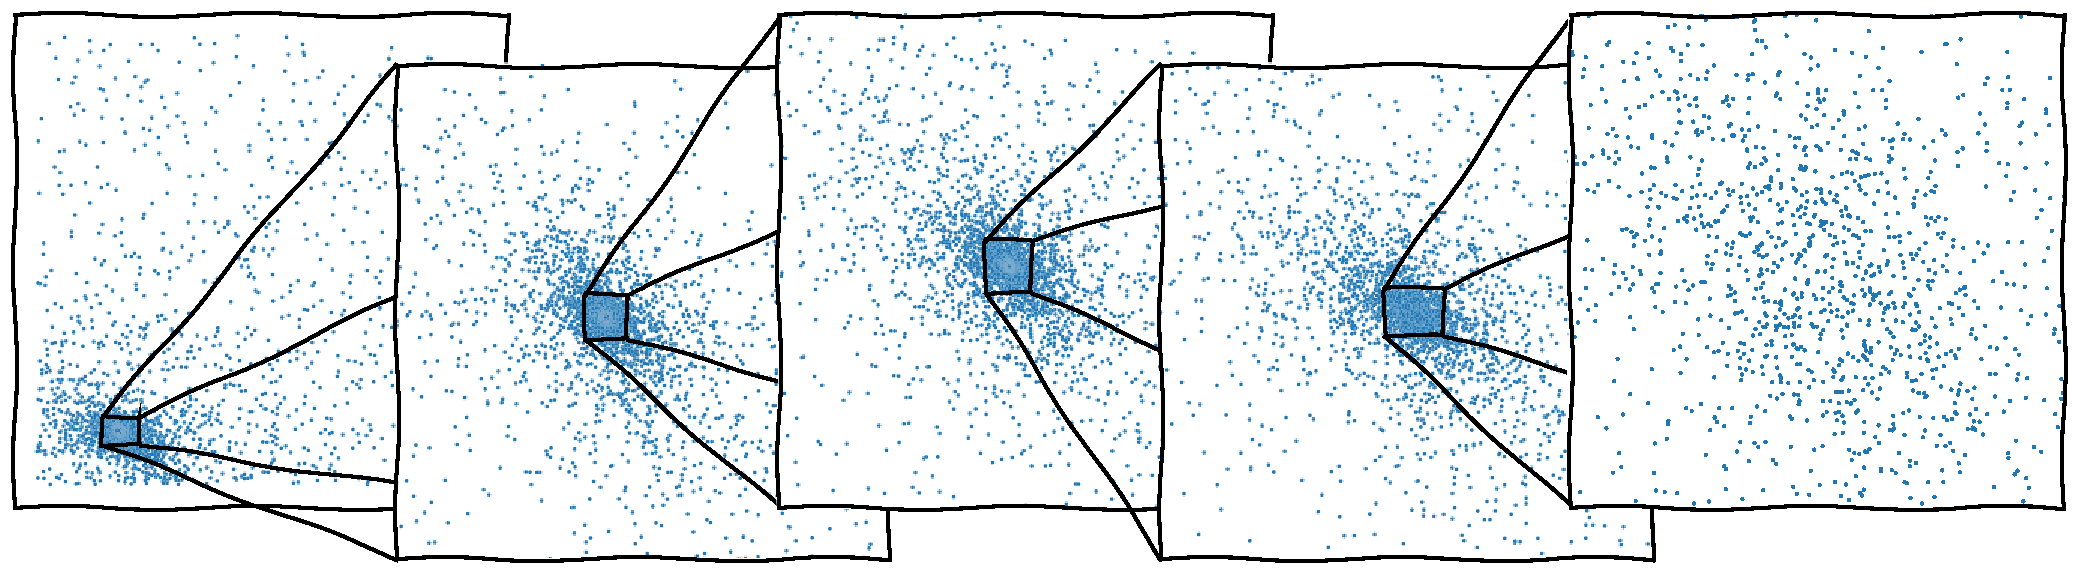
\includegraphics[width=\textwidth]{figures/dead_measure}
    \begin{columns}
        \column{0.69\textwidth}
        \begin{itemize}
            \item At the end, one is left with a set of discarded ``dead'' points.
            \item Dead points have a unique scale-invariant distribution $\propto\: \tfrac{dV}{V}$.
            \item Uniform over original region, exponentially concentrating on region of interest (until termination volume).
            \item Good for training emulators (HERA~\arxiv{2108.07282}).
        \end{itemize}
        \column{0.3\textwidth}
        \begin{block}{Applications}
        \begin{itemize}
            \item training emulators.
            \item gridding simulations
            \item beta flows
            \item ``dead measure'' 
        \end{itemize}
        \end{block}
    \end{columns}
\end{frame}

\begin{frame}
    \frametitle{The Challenge: Legacy vs Modern Paradigms}
    \begin{columns}
        \column{0.6\textwidth}
        \begin{block}{The Problem}
            \begin{itemize}
                \item Nested sampling viewed as \emph{legacy codebase}
                \item GPU-native paradigms dominating:
                    \begin{itemize}
                        \item Neural simulation-based inference
                        \item Modern JAX/PyTorch frameworks
                        \item Automatic differentiation \& JIT compilation
                    \end{itemize}
                \item Existing NS implementations:
                    \begin{itemize}
                        \item CPU-focused (Fortran, C++)
                        \item Limited vectorization
                        \item Difficult integration with ML workflows
                    \end{itemize}
            \end{itemize}
        \end{block}
        \column{0.4\textwidth}
        \begin{block}{The Solution}
            \begin{itemize}
                \item \textbf{Reformulate} nested sampling for GPU hardware
                \item \textbf{Vectorization} opportunities
                \item \textbf{Integration} with modern frameworks
                \item \textbf{State-of-the-art} performance
            \end{itemize}
        \end{block}
        \vspace{10pt}
        \centerline{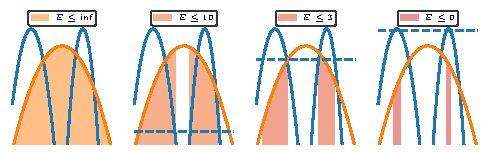
\includegraphics[width=0.8\textwidth]{figures/ns_diagram}}
    \end{columns}
\end{frame}

\begin{frame}
    \frametitle{Nested Sampling and Sequential Monte Carlo}
    \begin{columns}
        \column{0.5\textwidth}
        \begin{block}{Statistical Perspective}
            \begin{itemize}
                \item SMC: Rigorous statistical framework
                \item Rich theoretical foundation
                \item Nested sampling is a \emph{special case} of SMC
                \item Singular type of importance sampling
            \end{itemize}
        \end{block}
        \begin{block}{Physics Perspective}
            \begin{itemize}
                \item Nested sampling: Practical inference tool
                \item Direct evidence computation
                \item Model comparison focus
                \item Established in physical sciences
            \end{itemize}
        \end{block}
        \column{0.5\textwidth}
        \begin{block}{BlackJAX Integration}
            \begin{itemize}
                \item \textbf{Unified framework} for comparison:
                    \begin{itemize}
                        \item Nested sampling
                        \item HMC \& variants
                        \item SMC \& tempering
                        \item MALA, NUTS, etc.
                    \end{itemize}
                \item \textbf{Same GPU codebase} for all methods
                \item \textbf{Direct benchmarking} possible
                \item \textbf{Composable algorithms}
            \end{itemize}
        \end{block}
        \vspace{10pt}
        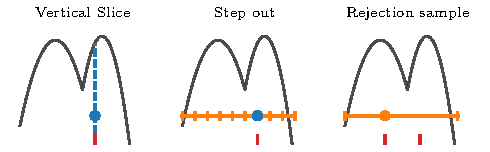
\includegraphics[width=\textwidth]{figures/slice_sampling_diagram}
    \end{columns}
\end{frame}

\begin{frame}
    \frametitle{BlackJAX Nested Slice Sampling}
    \begin{columns}
        \column{0.5\textwidth}
        \begin{block}{Core Algorithm}
            \begin{itemize}
                \item \textbf{Slice sampling} for constrained sampling
                \item Generate new live points: $\{\theta \sim \pi : \mathcal{L}(\theta) > \mathcal{L}_*\}$
                \item Vectorized operations across live points
                \item JAX transformations: \texttt{jit}, \texttt{vmap}, \texttt{grad}
            \end{itemize}
        \end{block}
        \begin{block}{GPU Advantages}
            \begin{itemize}
                \item \textbf{Parallel live points}: $n_{\text{live}} \sim 100\text{-}1000$
                \item \textbf{Vectorized slice sampling}
                \item \textbf{Batch likelihood evaluations}
                \item \textbf{Memory-efficient} on GPU
            \end{itemize}
        \end{block}
        \column{0.5\textwidth}
        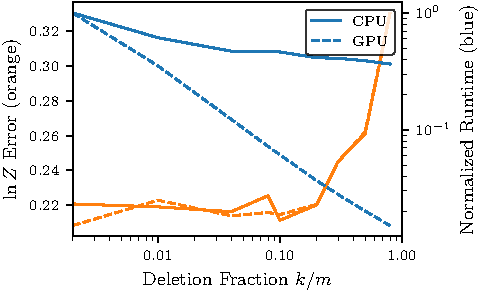
\includegraphics[width=\textwidth]{figures/scaling}
        \vspace{10pt}
        \begin{itemize}
            \item \textbf{Performance scaling}: Linear with $n_{\text{live}}$
            \item \textbf{GPU speedup}: $10\times$-$100\times$ vs CPU
            \item \textbf{Memory usage}: Constant per live point
        \end{itemize}
    \end{columns}
\end{frame}

\begin{frame}
    \frametitle{Performance Comparisons}
    \begin{columns}
        \column{0.5\textwidth}
        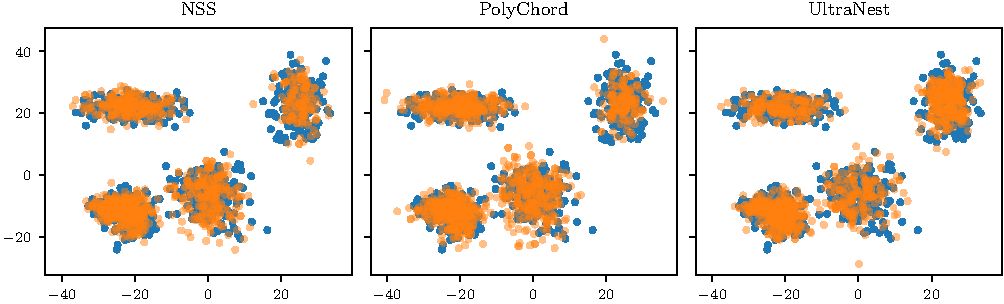
\includegraphics[width=\textwidth]{figures/pc_comparison}
        \vspace{5pt}
        \begin{itemize}
            \item Comparison with PolyChord (CPU)
            \item Same accuracy, faster convergence
            \item GPU memory efficiency
        \end{itemize}
        \column{0.5\textwidth}
        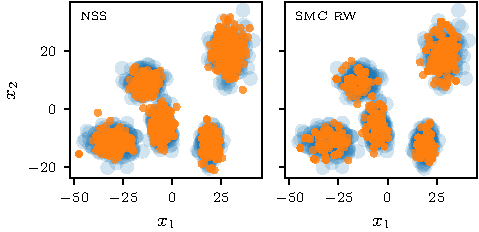
\includegraphics[width=\textwidth]{figures/mixture_gaussians_high_dim}
        \vspace{5pt}
        \begin{itemize}
            \item High-dimensional test problems
            \item Robust multimodal sampling
            \item Consistent evidence estimates
        \end{itemize}
    \end{columns}
\end{frame}

\begin{frame}
    \frametitle{Applications: Gravitational Wave Parameter Estimation}
    \student{david_yallup}{David Yallup}{PDRA}
    \begin{columns}
        \column{0.6\textwidth}
        \begin{itemize}
            \item \textbf{LIGO/Virgo data analysis}:
                \begin{itemize}
                    \item Binary merger parameter estimation
                    \item 15+ dimensional parameter spaces
                    \item Complex, multimodal posteriors
                    \item Real-time analysis requirements
                \end{itemize}
            \item \textbf{GPU advantages}:
                \begin{itemize}
                    \item Parallel waveform generation
                    \item Vectorized likelihood evaluations
                    \item $>10\times$ speedup for parameter estimation
                    \item Memory-efficient for long signals
                \end{itemize}
            \item \textbf{Evidence computation}:
                \begin{itemize}
                    \item Model comparison (GR vs modified gravity)
                    \item Detection vs noise discrimination
                    \item Population studies
                \end{itemize}
        \end{itemize}
        \column{0.4\textwidth}
        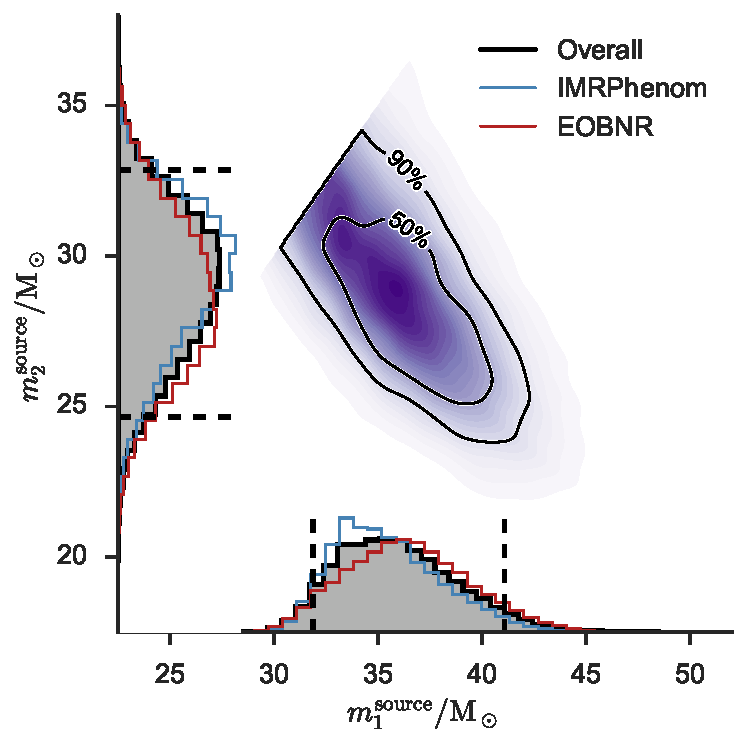
\includegraphics[width=0.49\textwidth]{figures/ligo_m1_m2}
        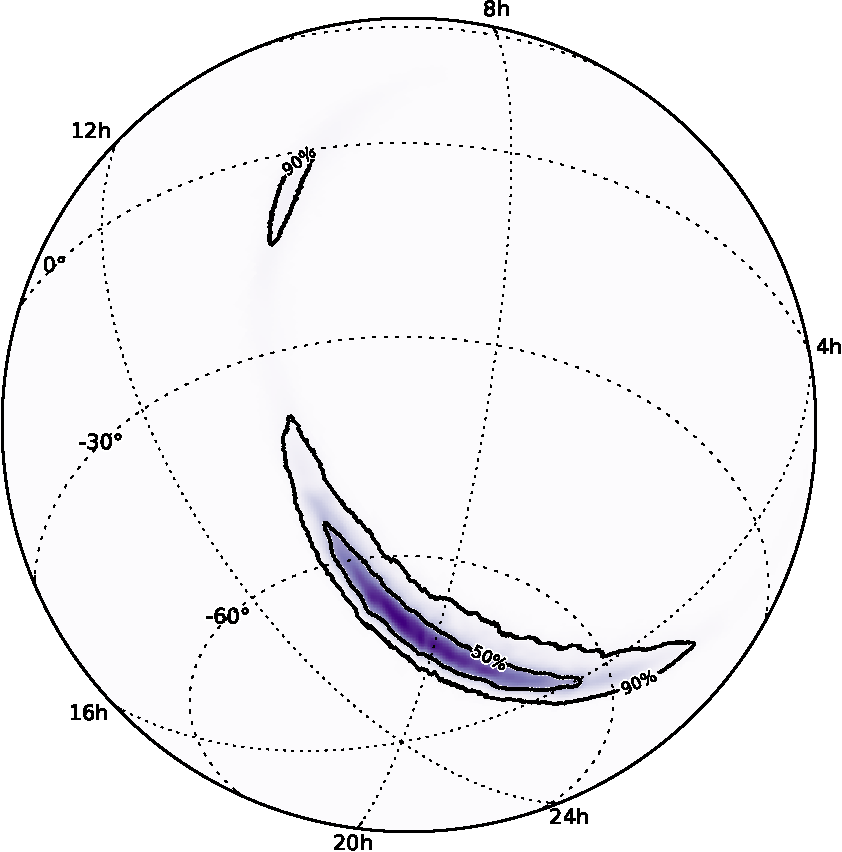
\includegraphics[width=0.49\textwidth]{figures/ligo_lambert-skymap}
        \vspace{10pt}
        \begin{itemize}
            \item Mass-mass posterior
            \item Sky localization
            \item Real-time follow-up enabled
        \end{itemize}
    \end{columns}
\end{frame}

\begin{frame}
    \frametitle{Applications: CMB Cosmology}
    \student{adam_ormondroyd}{Adam Ormondroyd}{PhD}
    \begin{columns}
        \column{0.55\textwidth}
        \begin{itemize}
            \item \textbf{Cosmological parameter inference}:
                \begin{itemize}
                    \item $\Lambda$CDM and extensions
                    \item 6-20+ dimensional parameter spaces
                    \item Non-Gaussian posteriors common
                    \item Model comparison critical
                \end{itemize}
            \item \textbf{GPU acceleration benefits}:
                \begin{itemize}
                    \item Vectorized $C_\ell$ computations
                    \item Parallel likelihood evaluations
                    \item Large survey data volumes
                    \item Systematic exploration of model space
                \end{itemize}
            \item \textbf{Tension quantification}:
                \begin{itemize}
                    \item CMB vs local universe measurements
                    \item Evidence ratios: $\mathcal{R} = \mathcal{Z}_{AB}/(\mathcal{Z}_A \mathcal{Z}_B)$
                    \item Suspiciousness calculations
                \end{itemize}
        \end{itemize}
        \column{0.45\textwidth}
        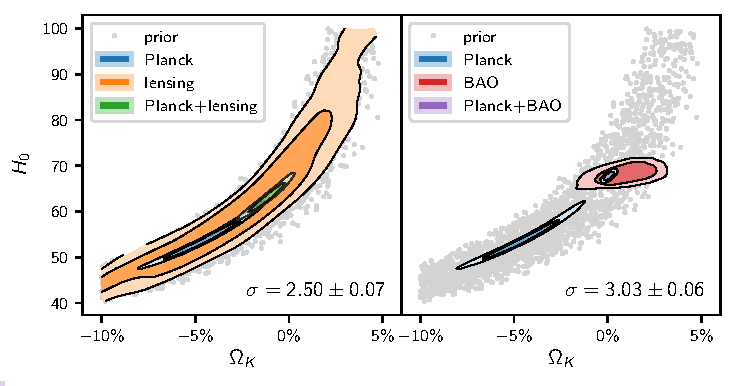
\includegraphics[width=\textwidth]{figures/omegak_H0_2}
        \vspace{5pt}
        \begin{itemize}
            \item Curvature-Hubble tension
            \item Non-Gaussian posteriors
            \item Model comparison essential
        \end{itemize}
    \end{columns}
\end{frame}

\begin{frame}
    \frametitle{Conclusions}
    \framesubtitle{\tthref{github.com/handley-lab/group}}
    \tikz[overlay,remember picture]
        \node[anchor=north east] (A) at ($(current page.north east)+(0,0)$) {
        
\includegraphics[width=0.09\textheight]{people/adam_ormondroyd.jpg}%
        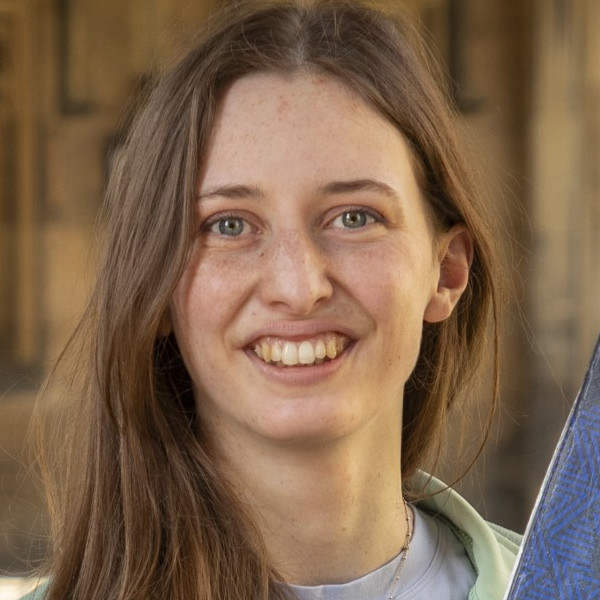
\includegraphics[width=0.09\textheight]{people/charlotte_priestley.jpg}%
        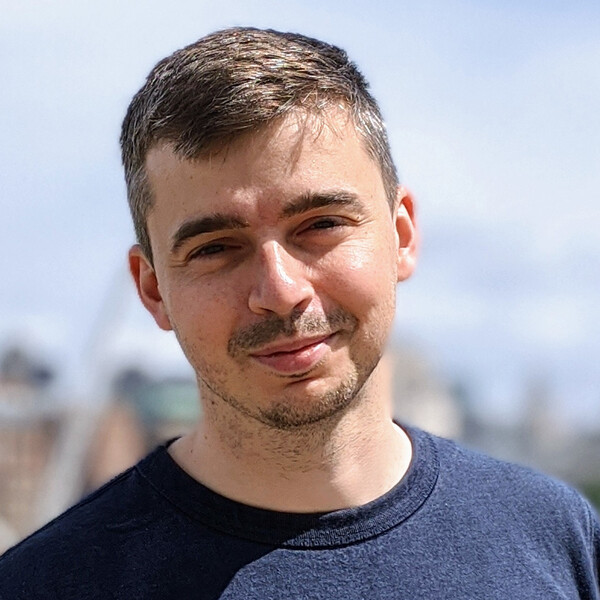
\includegraphics[width=0.09\textheight]{people/david_yallup.jpg}%
        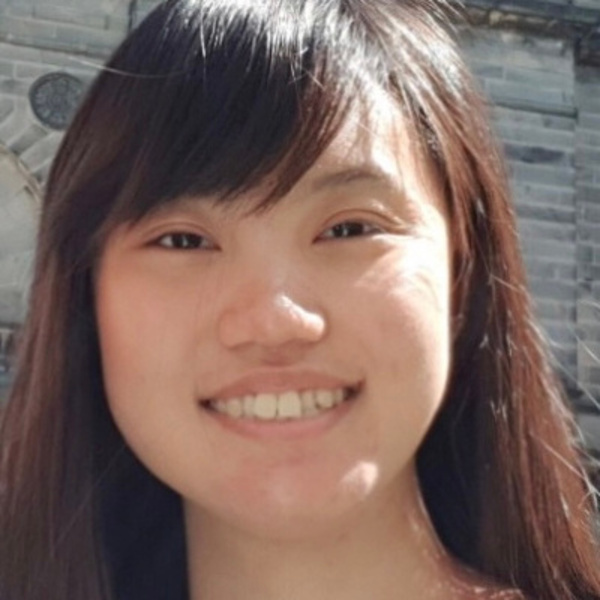
\includegraphics[width=0.09\textheight]{people/dily_ong.jpg}%
        
\includegraphics[width=0.09\textheight]{people/harry_bevins.jpg}%
        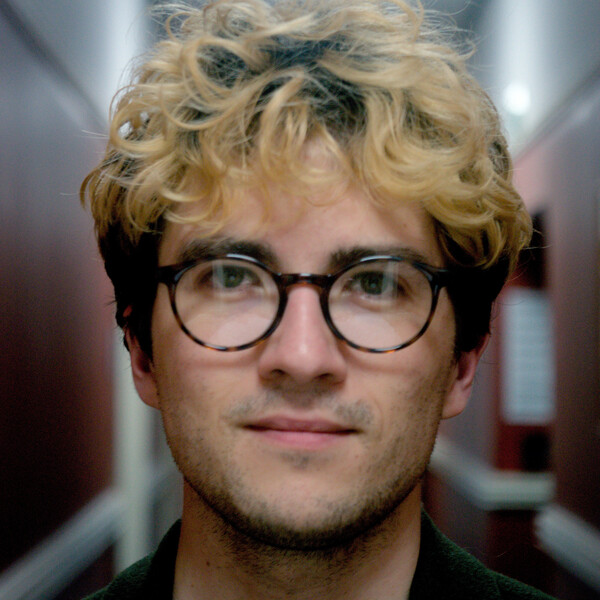
\includegraphics[width=0.09\textheight]{people/harvey_williams.jpg}%
        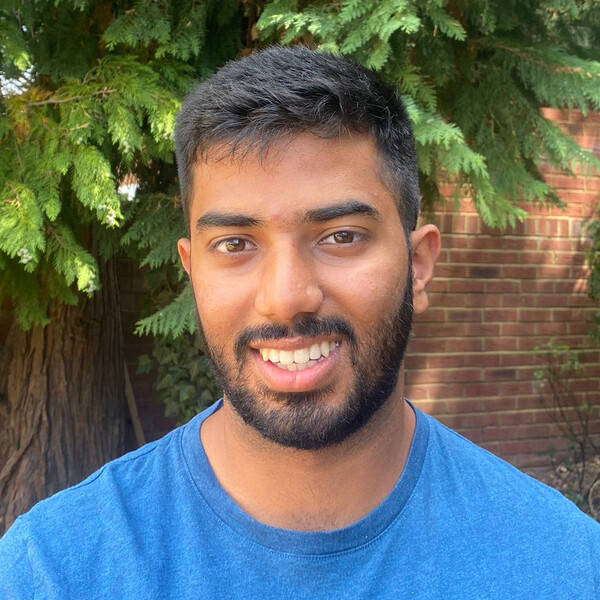
\includegraphics[width=0.09\textheight]{people/krish_nanavati.jpg}%
        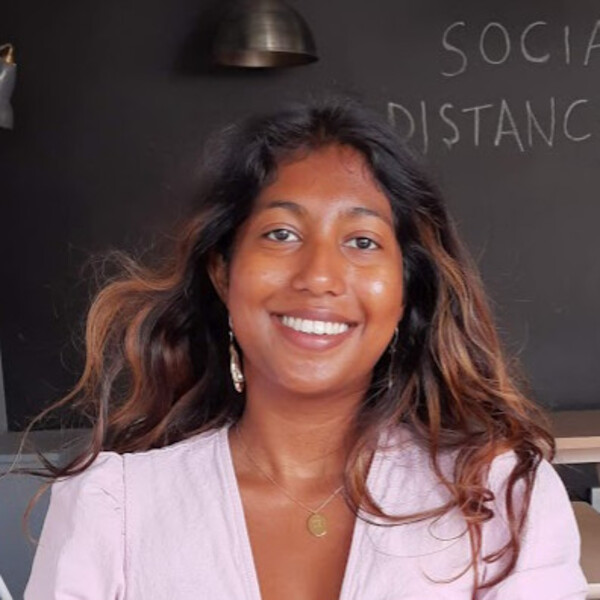
\includegraphics[width=0.09\textheight]{people/metha_prathaban.jpg}%
        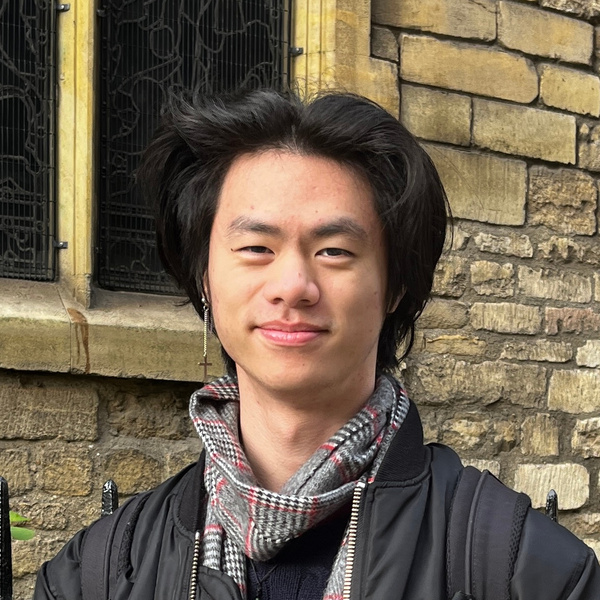
\includegraphics[width=0.09\textheight]{people/ming_yang.jpg}%
        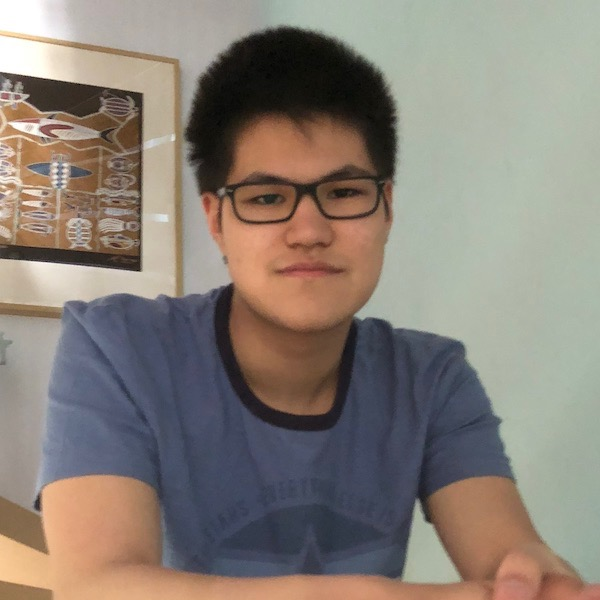
\includegraphics[width=0.09\textheight]{people/namu_kroupa.jpg}%
        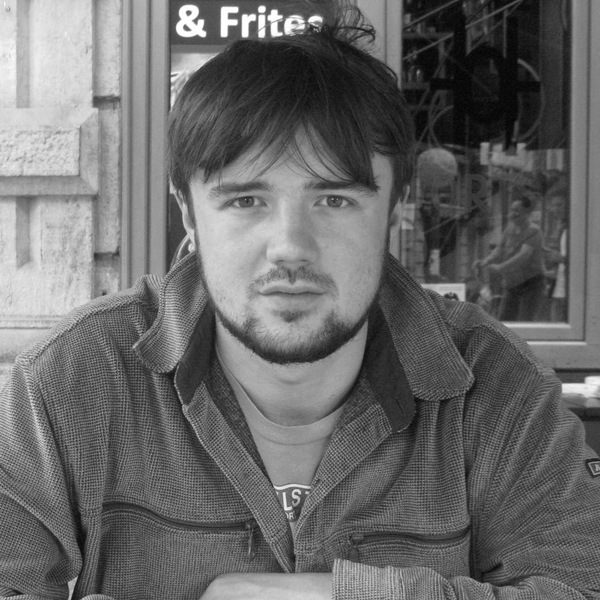
\includegraphics[width=0.09\textheight]{people/sam_leeney.jpg}%
        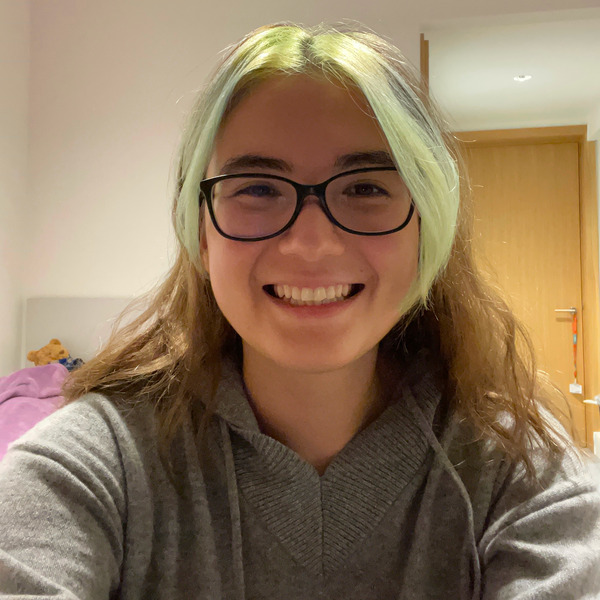
\includegraphics[width=0.09\textheight]{people/sinah_legner.jpg}%
        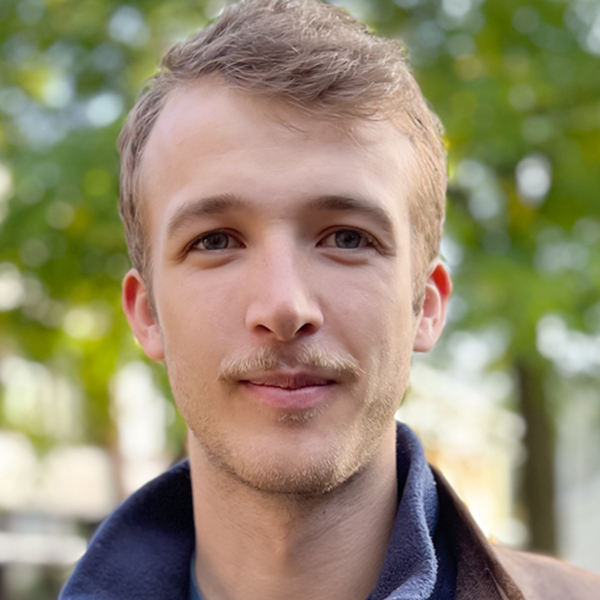
\includegraphics[width=0.09\textheight]{people/toby_lovick.jpg}%
        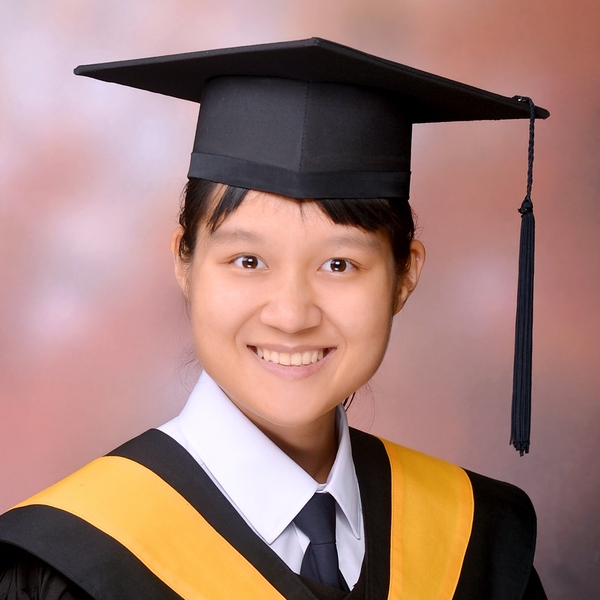
\includegraphics[width=0.09\textheight]{people/wei-ning_deng.jpg}%
        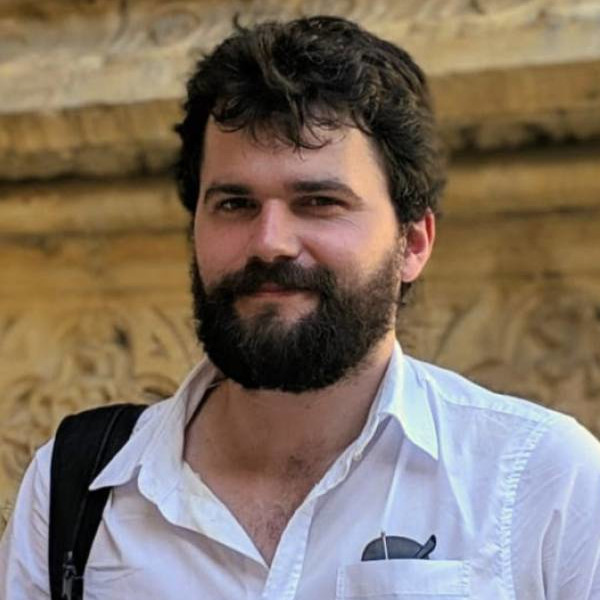
\includegraphics[width=0.09\textheight]{people/will_handley.jpg}%
        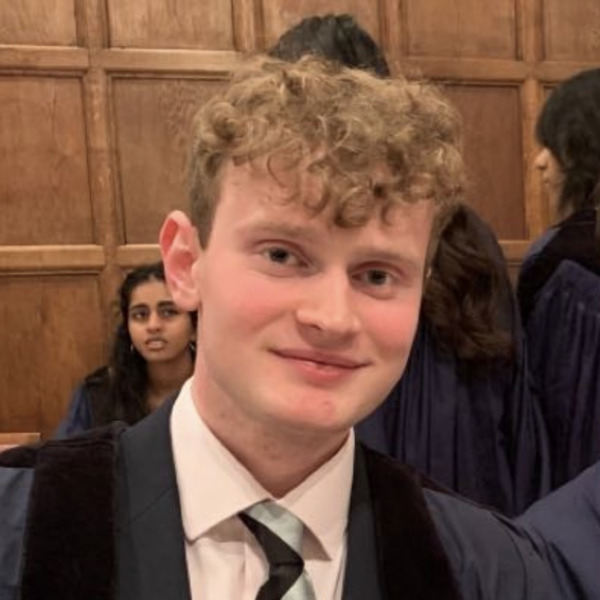
\includegraphics[width=0.09\textheight]{people/will_templeton.jpg}%
    };
\end{frame}

\end{document}
